\documentclass[pdftex,10pt,a4paper,twocolumn]{article}
\title{\textbf{Developing a cellular automaton model for kidney morphogenesis}}
\author{Ben Lambert}
\usepackage[titletoc,toc]{appendix}
\usepackage[pdftex]{graphicx}
\usepackage{url,times}
\usepackage{graphicx}
\usepackage{epstopdf}
\usepackage{amsmath}
\usepackage[all]{xy}
\usepackage{pxfonts}
\usepackage{colortbl}
\usepackage{color}
\usepackage{subfigure}
\usepackage{gensymb}
\usepackage{ctable}
\usepackage[justification=centering]{caption}[2007/12/23]
\usepackage{longtable}
\usepackage{pst-func}
\usepackage{pst-math}
\renewcommand{\bibname}{Works Cited}
\usepackage{listings}
\usepackage{setspace}
\usepackage{algorithm}
\usepackage{bbm}

\newcommand{\HRule}{\rule{\linewidth}{0.5mm}}
\begin{document}

\twocolumn[
\maketitle
\doublespacing
\begin{@twocolumnfalse}
\begin{abstract}
The development of the kidney involves the interaction between two distinct populations of cells: the metanephric mesenchyme and the epithelium of the Wolffian Duct. From E10.5-11 (in mouse organ cultures) a uretic bud (UB) of epithelium forms, which invades the space of the mesenchyme; later undergoing branching and extension which ultimately results in the components of a functioning kidney: the nephrons and collecting duct. In this paper a simple cellular automaton model is presented which recapitulates the initial emergence of the UB, along with its primary branching. In the model, metanephric mesenchyme cells release a chemo-stimulant GDNF (implicated from experiments), which diffuses throughout the simulation area, and is taken up by the epithelium cells, influencing their resultant behaviour.
\end{abstract}
\end{@twocolumnfalse}
]

\section{Introduction}
The human kidney's primary function is to filter blood of waste products (mainly urea) from metabolism. The most important functional units of a kidney are nephrons, which are responsible for regulating the concentration of water and other solutes released in urine. In a nephron blood is filtered by the Glomerulus, and the filtrate then flows through a system of structures (the proximal tubule, loop of Henle and the distal tubule), where filtrates are selectively reabsorbed, then connects with a connecting duct which delivers the waste products to the ureter for excretion.

A fully developed human kidney is composed of 200,000 to 1.8 million nephrons, connected by a system of connecting ducts to the ureter, with the majority of the structure being formed during the embryonic stages of life ~\cite{hughson2003glomerular}. There are functional consequences for reduced nephron number, with evidence suggesting that this can cause hypertension and renal failure in adult life ~\cite{hoy2008nephron}. Furthermore, kidney and urinary tract congenital disorders are amongst the most common birth defects ~\cite{airik2007down}, with hypoplasia and dysplasia occurring in up to 1/200 births \cite{weber2006prevalence}. These are suggestive that biological and computational models which can help illuminate the cause, action and potential remedy of these types of disorder would be of value clinically.

Experimental work has focussed on animal models (mice, rats and fish) to study renal development. Broadly, there are two categories of experiment which have been undertaken: \textit{in vivo} studies of the effects of knock-out genes, and \textit{in vitro} studies of explanted kidney cells, grown in particular culture media. In particular, mouse studies have already demonstrated their relevance to the study of human kidneys. Dominant renal hypodysplastic kidneys, characteristic of a number of human renal disorders, display mutations in genes which were first discovered in the mouse ~\cite{LittleMMcMahon2012}.

During embryogenesis the early kidney is made up solely of undifferentiated cells, called the intermediate mesoderm (IM). These cells act as progenitors for all future nephron cells and collecting duct epithelium. At E9.5 in mouse studies the cells at the dorsal end of the organ form the epithelium of the Wolffian Duct extending in a rostro-caudal direction, with the rest of the cells maintaining their respective pluripotency ~\cite{CostantiniFKopan2010},\cite{saxen1987early}. Later on during development the remaining intermediate mesoderm becomes specialised along the rostro-caudal axis, with a relatively dense 'cloud' of mesenchyme forming at the caudal end ~\cite{CostantiniFKopan2010}, called the metanephric mesenchyme (MM).

At E10.5-11, due to factors released by the MM, there is an outgrowth of the epithelium, taking the form of a single discrete bud - the uretic bud (UB) - in normal organ development, which invades the MM ~\cite{CostantiniFKopan2010},\cite{LittleMMcMahon2012}. The UB then undergoes rounds of branching and extension, resulting in the branched structure of the collecting duct and its associated tubules. During this time, there are a nexus of reciprocal interactions which determine the specific nature of the branched structure. Factors produced by the epithelium also have a role to play in determining nephronic strcuture. In particular Wnt9b has been implicated in stimulating differentiation of mesenchymal cells proximal to the UB to form epithelium which acts as progenitors to nephrons. Normal development of the kidney's underlying structure stops at around parturition.

\section{GDNF stimulation of uretic bud growth}
There are a number of chemical signals produced by the metanephric mesenchyme which stimulate the growth of the uretic bud into the space occupied by the MM, and these have been reviewed comprehensively~\cite{costantini2006gdnf}, Dressler ~\cite{dressler2006cellular}. One of the most important of these factors is glial derived neurotrophic factor (GDNF), as GDNF$^{--}$ mutant mice typically do not produce uretic buds. Furthermore, this factor is the morphogen associated with driving the branching of the uretic bud.

GDNF is produced by the MM, and acts paracrinally on the epithelium; likely binding with two membrane surface Ret receptors (along with a co-receptor GFR$\alpha 1$) ~\cite{MenshykauDIber}. Ret$^{--}$ mice, like GDNF$^{--}$ mutants, (as well as GFR$\alpha 1$$^{--}$), fail to develop uretic buds ~\cite{CostantiniFKopan2010},\cite{majumdar2003wnt11},\cite{treanor1996characterization}, suggesting that a pathway involving these factors is involved in inducing the initial growth of the epithelium into the MM.

The chemo-attractive characteristics of GDNF ~\cite{tang2002ureteric},\cite{tang1998ret}, have led some to suggest that initial growth of uretic bud, as well as subsequent branching, is due, in part, to growth and movement of epithelium towards local GDNF sources \cite{sariola2003novel}. Furthermore, explanted epithelium cells have also been shown to grow additional uretic buds in the presence of beads soaked in GDNF \cite{pepicelli1997gdnf}. 

Ret has been shown to upregulate its own expression, as well as production of Wnt11 by the epithelium cells \cite{pepicelli1997gdnf}, which then regulates production of GDNF by the metanephric mesenchyme cells ~\cite{majumdar2003wnt11}. Thus production of GDNF exists in a feed-forward network, with reciprocal interactions between the epithelium and the mesenchyme cells. These interactions are displayed visually in figure \ref{fig:pathways}. GDNF expression is however tempered by a negative feedback loop involving \textit{Sprouty1} ~\cite{basson2005sprouty1}. FGF proteins have also been implicated in stimulating the emergence of the initial uretic bud, as well as branching, although it is likely that this process is less important than the GDNF mechanism, since FGFR2${^{--}}$ still undergo branching, albeit at a reduced level ~\cite{sims2009three}. However, in \textit{Sprouty1}${^{--}}$ mice, hyper-expression of FGF signalling proteins can generate phenotypically normal kidneys in GDNF$^{--}$ and Ret$^{--}$ mutants; which otherwise would have failed to develop kidneys at all. Since both Ret/GDNF and FGF10/FGFR have the same downstream targets ETV4/ETV5, it is likely that they may fulfil similar functions. This sort of redundancy could potentially have benefits evolutionarily.

\begin{figure*}[t] 
\centering
\scalebox{0.35} 
{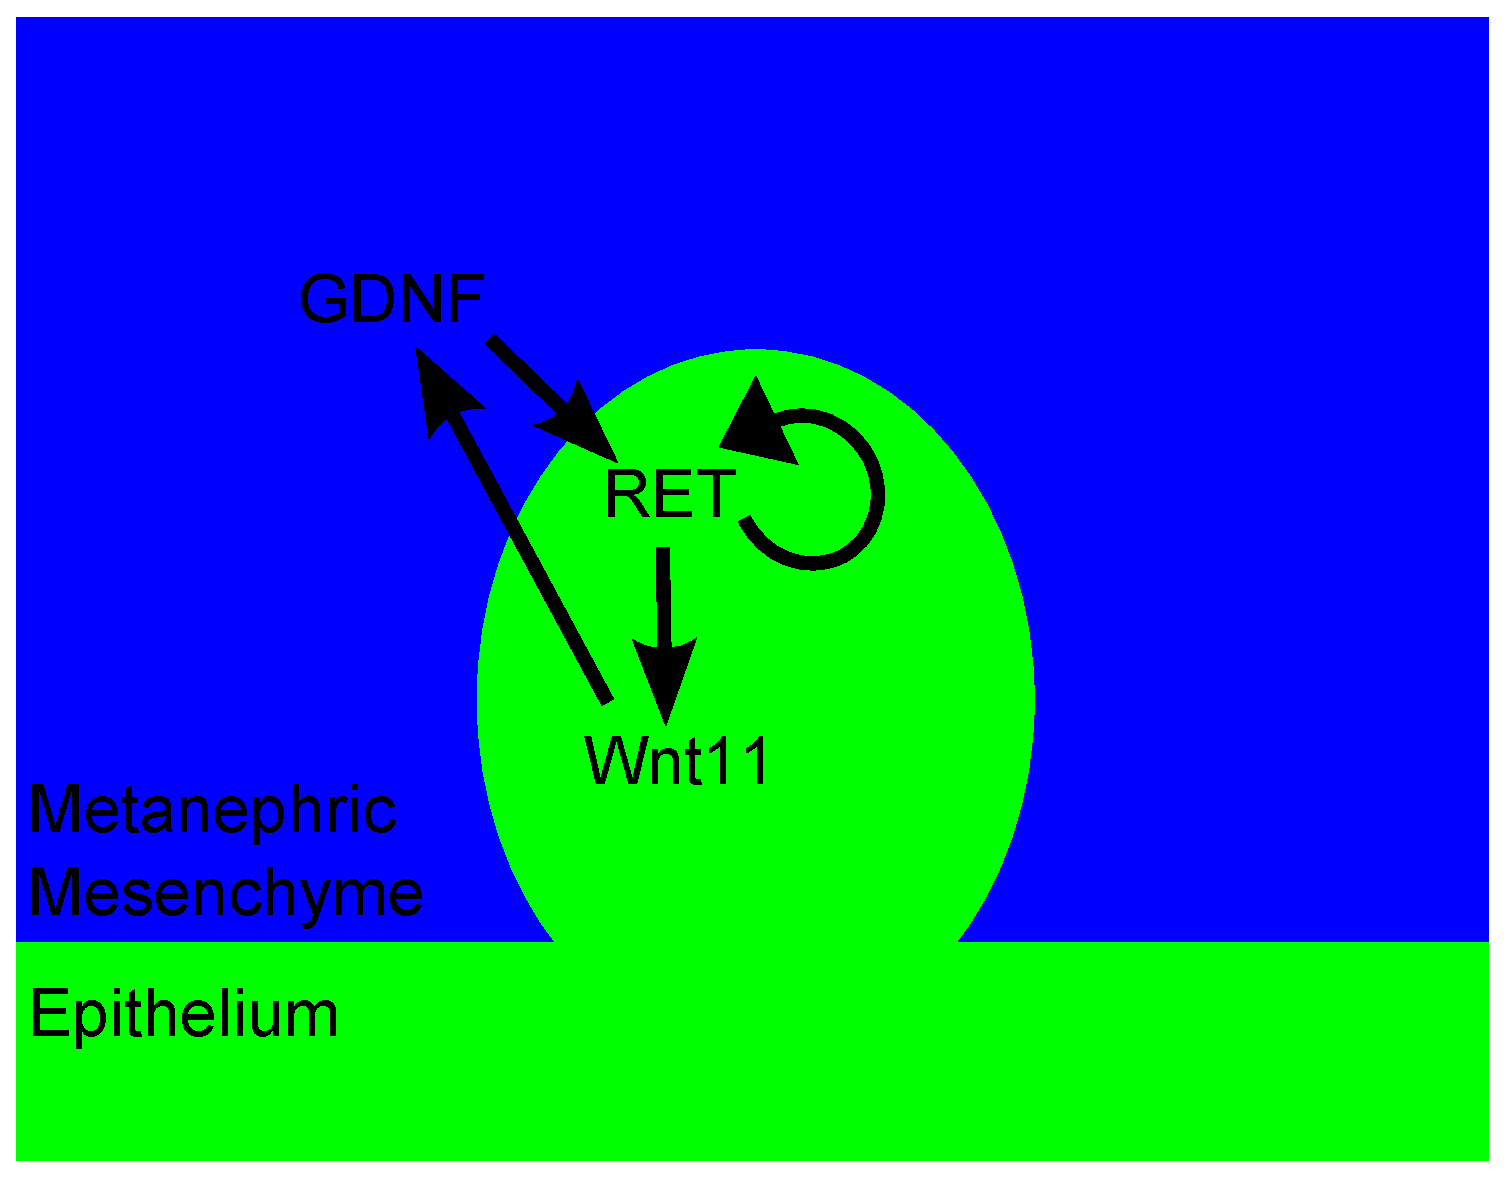
\includegraphics{pathways.eps}}
\caption{Shows the dominant reaction pathway for the regulation of GDNF in the developing kidney.}\label{fig:pathways}
\end{figure*} 

\section{Branching hypotheses}
When the UB has invaded the MM, the UB undergoes approximately ten rounds of branching ~\cite{srinivas1999expression}. Subsequent to the initial branching, there is notable collecting duct lengthening, with one-two final rounds of branching before parturition ~\cite{cebrian2004morphometric}.

Branching of an emergent UB tip is witnessed in the absence of mesenchyme in explanted epithelium cells ~\cite{qiao1999branching}, however it is important to note that a culture medium containing GDNF, as well as medium derived from cells from the early metanephric mesenchyme are required for this to occur. Also, the branching morphology obtained with \textit{in vitro} explants is not the same as \textit{in vivo} patterning, suggesting that the mesenchyme-epithelium interaction at least plays a supporting role in kidney morphogenesis. However, this result is suggestive that an important mechanism for branching is cell-contact-independent.

The mechanisms which lead to the observed branching of epithelium in both \textit{in vivo} and \textit{in vitro} experiments is not well understood. The simplest hypothesis is that branching occurs as a result of local maxima and minima in GDNF, with epithelium cells 'attracted' towards the former \cite{sariola2003novel}.



\section{Differentiation of mesenchyme into nephron progenitors}

\section{Model formulation}

\section{Results}

\section{Discussion}

\section{Conclusion}
\bibliographystyle{plain}
\bibliography{Kidney}


\end{document}